% Digital Logic Report Template
% Created: 2020-01-10, John Miller
%==========================================================
%=========== Document Setup  ==============================
% Formatting defined by class file
\documentclass[11pt]{article}
% ---- Document formatting ----
\usepackage[margin=1in]{geometry}  % Narrower margins
\usepackage{booktabs}                    % Nice formatting of tables
\usepackage{graphicx}                    % Ability to include graphics
%\setlength\parindent{0pt}    % Do not indent first line of paragraphs 
\usepackage[parfill]{parskip}      % Line space b/w paragraphs
%     parfill option prevents last line of pgrph from being fully justified
% Parskip package adds too much space around titles, fix with this
\RequirePackage{titlesec}
\titlespacing\section{0pt}{8pt plus 4pt minus 2pt}{3pt plus 2pt minus 2pt}
\titlespacing\subsection{0pt}{4pt plus 4pt minus 2pt}{-2pt plus 2pt minus 2pt}
\titlespacing\subsubsection{0pt}{2pt plus 4pt minus 2pt}{-6pt plus 2pt minus 2pt}
% ---- Hyperlinks ----
\usepackage[colorlinks=true,urlcolor=blue]{hyperref} % For URL's. Automatically 
%links internal references.
% ---- Code listings ----
\usepackage{listings}                          % Nice code layout and inclusion
\usepackage[usenames,dvipsnames]{xcolor} % Colors (needs to be defined before 
%using colors)
% Define custom colors for listings
\definecolor{listinggray}{gray}{0.98}          % Listings background color
\definecolor{rulegray}{gray}{0.7}              % Listings rule/frame color
% Style for Verilog
\lstdefinestyle{Verilog}{
language=Verilog,                        % Verilog
backgroundcolor=\color{listinggray},     % light gray background
rulecolor=\color{blue},                  % blue frame lines
frame=tb,
% lines above & below
linewidth=\columnwidth,                  % set line width
basicstyle=\small\ttfamily,   % basic font style that is used for the code
breaklines=true,                         % allow breaking across 
%columns/pages
tabsize=3,
% set tab size
commentstyle=\color{gray},    % comments in italic 
stringstyle=\upshape,                    % strings are printed in normal 
%font
showspaces=false,                        % don't underscore spaces
}
% How to use: \Verilog[listing_options]{file}
\newcommand{\Verilog}[2][]{%
\lstinputlisting[style=Verilog,#1]{#2}
}







%======================================================
%=========== Body  ====================================
\begin{document}
\title{ELC 2137 Lab 10: 7-segment Display with Time-Division Multiplexing}
\author{Justin Woods}
\maketitle

\section*{Summary}

\section{Questions}

\begin{enumerate}
	\item How should I format them?
	Use the same numbered list format as in the assignment (like this).
	\item Do I need to include the original question?
	Yes, include both the question and the answer to it.
	\item Should I put the question on the first line?
	Yes, then skip a line and write your answer.  This produces a nicely 
	formatted result.
\end{enumerate}

\section*{Results}

\begin{figure}[ht]\centering
	
	\begin{tabular}{l|rrrrrrrrrrr}	
		Time (ns): & 0-5 & 5-10 & 10-15 & 15-20 & 20-25 & 25-30 & 30-35 & 35-40 & 40-45 & 45-50 & 50 55 \\
		\midrule
		D (hex) & 0 & 0 	  & A & A & 3 	    & 3 	  & 0 	    & 0 & 0$\to$6 & 6 & 6 \\
		clk     & 0 & 1 	  & 0 & 1 & 0 	    & 1 	  & 0 	    & 1 & 0 	  & 1 & 0 \\
		en  	& 0 & 0 	  & 1 & 1 & 1$\to$0 & 0$\to$1 & 1$\to$0 & 0 & 0$\to$1 & 1 & 1 \\
		rst 	& 0 & 0$\to$1 & 0 & 0 & 0 		& 0 	  & 0		& 0 & 0		  & 0 & 0 \\
		\midrule
		Q(hex) 	& X & 0$\to$0 & 0 & A & A 		& A 	  & A 		& A & A 	  & 6 & 6 \\
		\bottomrule
	\end{tabular}
	\bigskip
	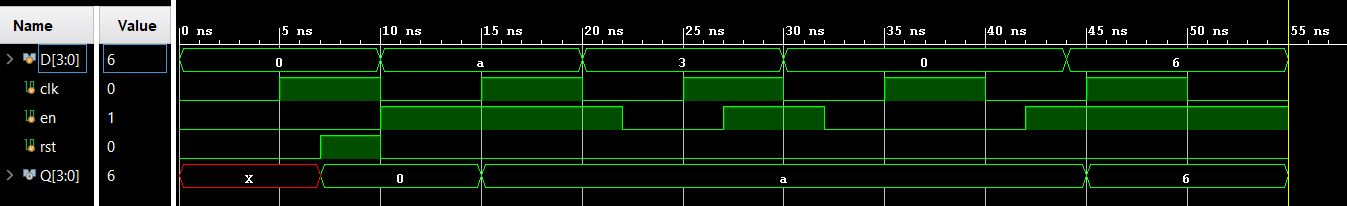
\includegraphics[width=1\textwidth,angle=0,origin=c]{registerWaveform}
	\caption{Register Simulation Waveform and ERT}
	\label{fig:sim_with_table}
\end{figure}

\begin{figure}[ht]\centering
	
	\begin{tabular}{l|rrrrrr}
		Time (ns): & 0-10 & 10-20 & 20-30 & 30-40 & 40-50 & 50-60 \\
		\midrule
		in0 & 4  & 14& 1 & 1 & 1 & 8 \\
		in1 & 10 & 5 & 0 & 0 & 1 & 0 \\
		op  & 0  & 1 & 2 & 3 & 4 & 5 \\
		\midrule
		out & E  & 9 & 0 & 1 & 0 & 8 \\
		\bottomrule
	\end{tabular}
	\bigskip
	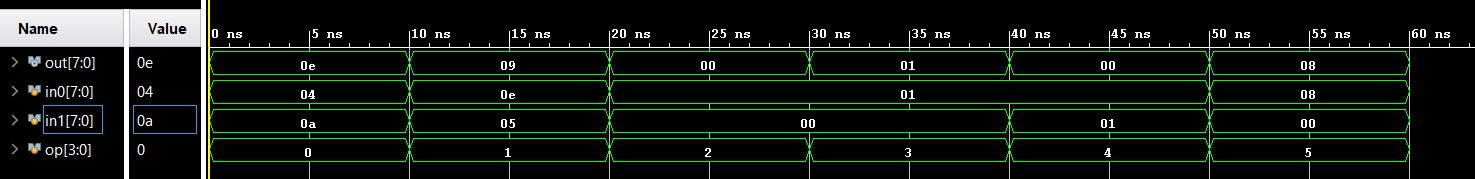
\includegraphics[width=1\textwidth,angle=0,origin=c]{aluWaveform}
	\caption{ALU Simulation Waveform and ERT}
	\label{fig:sim_with_table}
\end{figure}

\begin{figure}[ht]\centering
	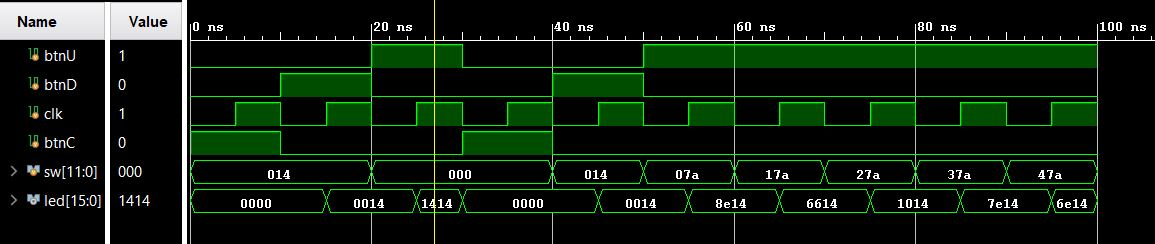
\includegraphics[width=1\textwidth,angle=0,origin=c]{toplevelWaveform}
	\caption{Top Level Waveform}
	\label{fig:sim_with_table}
\end{figure}
	\clearpage

\section*{Code}

\begin{lstlisting}[style=Verilog,
caption=Register Source Code,
label=MUX w/ two inputs Source Code
]
	module register #(parameter N=1) 
		(
		input clk, rst, en, input [N-1:0] D,
		output reg [N-1:0] Q
		);
		
		always @(posedge clk, posedge rst) 
		begin
			if (rst==1)
				Q <= 0 ;
			else if (en==1)
				Q <= D ;
		end
	endmodule
\end{lstlisting}

\begin{lstlisting}[style=Verilog,
caption=Register Test,
label=MUX2 Test
]
	module registerTEST();
	
		reg [3:0] D;
		reg clk, en, rst;
		wire [3:0] Q;
		
		register #(.N(4)) r(.D(D), .clk(clk),
			.en(en), .rst(rst),
			.Q(Q) );
		
		always begin 
			clk = ~clk; #5; 
		end
		
		// this block only runs once
		initial begin
			clk=0; en=0; rst=0; D=4'h0; #7;
			rst = 1; #3;
			// reset
			D = 4'hA; en = 1; rst = 0; #10;
			D = 4'h3;   #2;
			en = 0;     #5;
			en = 1;     #3;
			D = 4'h0;   #2;
			en = 0;     #10;
			en = 1;     #2;
			D = 4'h6;   #11;
			$finish;
		end 
	endmodule
\end{lstlisting}

\clearpage
\begin{lstlisting}[style=Verilog,
caption=ALU Source Code,
label=MUX w/ four inputs Source Code
]
	module alu #(parameter N=8) 
		( 
		output reg[N-1:0] out,
		input [N-1:0] in0,
		input [N-1:0] in1,
		input [3:0] op 
		);
		
		// Local parameters
		parameter ADD =0; 
		parameter SUB =1; 
		parameter AND =2; 
		parameter OR  =3; 
		parameter XOR =4;
		
		always @* 
		begin 
			case(op)
				ADD: out = in0 + in1;
				SUB: out = in0 - in1;
				AND: out = in0 & in1;
				OR: out = in0 | in1;
				XOR: out = in0 ^ in1;
				default: out = in0;
			endcase
		end
	endmodule
\end{lstlisting}

\begin{lstlisting}[style=Verilog,
caption=ALU Test,
label=MUX4 Test
]
	module aluTEST();
	
		wire[7:0] out;
		reg [7:0] in0, in1;
		reg [3:0] op;
		
		alu #(.N(8)) a(.in0(in0), .in1(in1), .op(op),
			.out(out) );
		
		initial begin
			op = 0; in0 = 4; in1 = 10; #10			
			op = 1; in0 = 14; in1 = 5; #10			
			op = 2; in0 = 1; in1 = 0; #10			
			op = 3; in0 = 1; in1 = 0; #10
			op = 4; in0 = 1; in1 = 1; #10
			op = 5; in0 = 8; in1 = 0; #10
			$finish;  
		end          
	endmodule
\end{lstlisting}
\clearpage
\begin{lstlisting}[style=Verilog,
caption=Top Level Source Code,
label=Anode Decoder Source Code
]
	module top_lab9(
		input btnU, btnD, clk, btnC,
		input [15:0]sw,
		output [15:0] led
		);
	
		wire [7:0]reg1out, a1out, reg2out;
		
		register #(.N(8)) reg1 (.D(sw[7:0]), .clk(clk),
			.en(btnD), .rst(btnC),
			.Q(reg1out) ); 
		
		alu #(.N(8)) a1 (.in1(reg1out), .in0(sw[7:0]), .op(sw[11:8]),
			.out(a1out) ); 
		
		register #(.N(8)) reg2 (.D(a1out), .clk(clk),
			.en(btnU), .rst(btnC),
			.Q(reg2out) );
			
		assign led[7:0] = reg1out;
		assign led[15:8] = reg2out;
	
	endmodule
\end{lstlisting}


\end{document}